\chapter{Machine and Deep Learning} \label{sec:ml}

The modern world is overflowing with data. It has reached a stage where humans can no longer regulate it since the rate of analysis is far slower than the continuous growth of data. According to Figure~\ref{fig:volume_of_data}, this rapid growth is not expected to stop anytime soon, so tools and technologies are needed to make the process of making sense of data more efficient.

\begin{figure}[htbp]
    \centering
    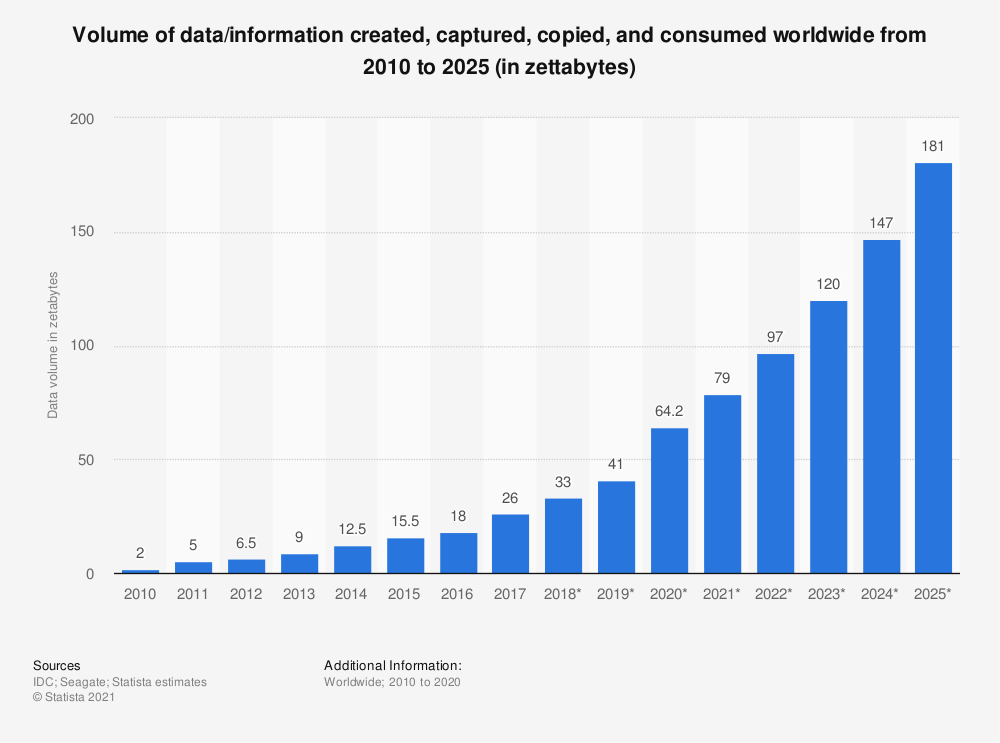
\includegraphics[width=0.85\linewidth]{volume_of_data.png}
    \caption{The volume of data created, captured, copied, and consumed from 2010 to 2025~\cite{TotalStatista}}
    \label{fig:volume_of_data}
\end{figure}

\gls{ML}, which is a subfield of artificial intelligence and computer science, is a promise that humans will be able to extract useful information from all these data. It focuses on using data and algorithms to imitate the way humans learn while improving accuracy~\cite{IBMCloudEducationWhatLearning}.

For a long time, one of the major differences between humans and computers has been that humans tend to naturally improve their approach to solving problems by learning from their mistakes and trying to fix them. Traditional computer programs are unable to improve their behavior since they do not consider the outcome of their job~\cite{Luckert2016UsingDocuments}. 

This topic is addressed by \gls{ML}, which entails the development of computer systems that can learn and improve their performance by accumulating more data and experience. A. Samuel was the first scientist to design a self-learning program in 1952 when he developed a program that improved at playing checkers as the number of games increased~\cite{Samuel1959SomeCheckers,Luckert2016UsingDocuments}. 

\gls{ML} relies solely on the availability of the data and does not need any rule-based programming. There is a distinction to be made between traditional programming and \gls{ML}. In traditional programming, data and programs are sent as inputs to the machine, and it produces an output, whereas in \gls{ML}, data and outputs are inputs to the system, and the machine's output is the program that has been learned to make predictions on unknown examples. The primary difference between traditional programming and \gls{ML}'s approach is represented in Figure~\ref{fig:tradition_vs_ml}.

\begin{figure}[htbp]
    \centering
    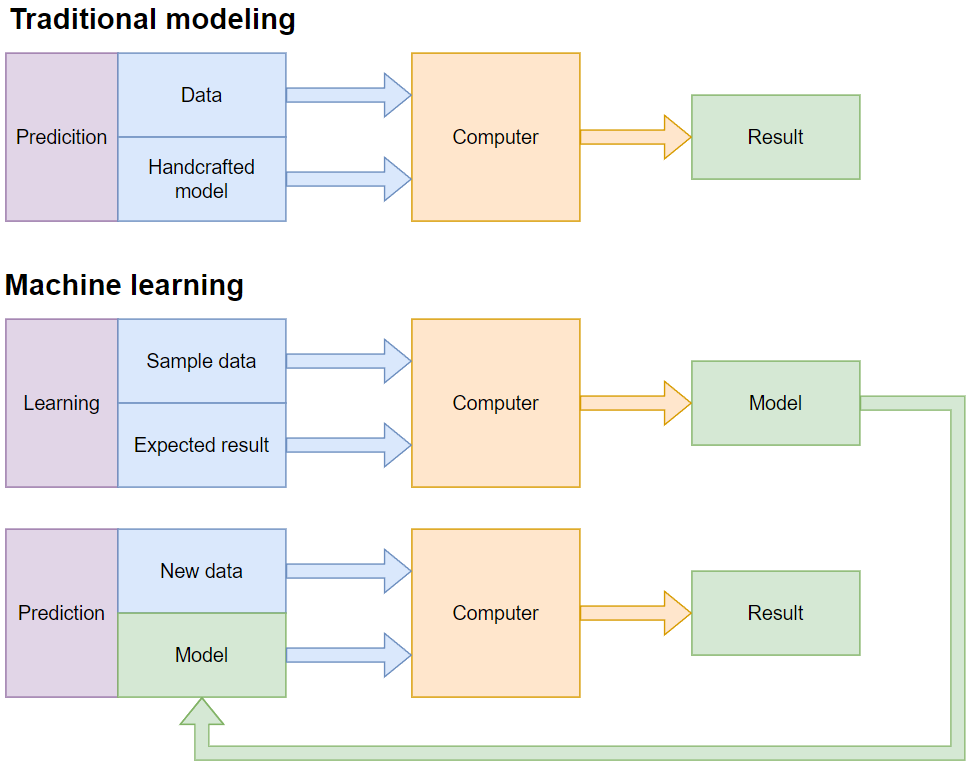
\includegraphics[width=0.75\linewidth]{tradition_vs_ml}
    \caption{Difference between Traditional Programming and Machine Learning. Adapted from~\cite{Kassel2017PredictingAzavea}}
    \label{fig:tradition_vs_ml}
\end{figure}

\begin{figure}[htbp]
    \centering
    \includegraphics[width=0.75\linewidth]{Chapters/Figures/tradition_vs_ml2.pdf}
    \caption{Difference between Traditional Programming and Machine Learning. Adapted from~\cite{Kassel2017PredictingAzavea}}
    \label{fig:tradition_vs_ml}
\end{figure}

To understand better the concepts of \gls{ML}, Table~\ref{tab:ml_terminologies} provides a few important terminologies.

\begin{table}[ht]
	\caption{Machine Learning concepts~\cite{MachineDevelopers}}
	\label{tab:ml_terminologies}
\centering
\begin{tabular}{p{2.5cm}c}
	\toprule
	\multicolumn{1}{c}{\textbf{Concept}} & \textbf{Description} \\
	\midrule
	
	Dataset
    & 
    \begin{tabular}[c]{@{}c@{}}
        Collection of data. In tabular data, each column represents a\\
        feature and each row represents a given record of the data set\\
        in question. Instead of tables, datasets can also consist of a\\
        collection of files.
    \end{tabular} 
    \\\midrule
	
    Model
    & 
    \begin{tabular}[c]{@{}c@{}}
        Representation of a \gls{ML} system after it has learnt\\
        from the training data.
    \end{tabular} 
    \\\midrule
    
    Feature
    & 
    \begin{tabular}[c]{@{}c@{}}
        Measurable characteristic of the dataset.
    \end{tabular} 
    \\\midrule
    
    Feature Vector
    & 
    \begin{tabular}[c]{@{}c@{}}
        Multiple features are used as an input to the \gls{ML} model.
    \end{tabular} 
    \\\midrule
    
    Training
    & 
    \begin{tabular}[c]{@{}c@{}}
        %Procedure for obtaining a model's optimum parameters.
        Procedure for obtaining appropriate values for model weights and bias (parameters).
    \end{tabular} 
    \\\midrule
    
    Parameter
    & 
    \begin{tabular}[c]{@{}c@{}}
        Model variable that is self-taught by the \gls{ML} system.
    \end{tabular} 
    \\\midrule
    
    Prediction
    & 
    \begin{tabular}[c]{@{}c@{}}
        Once the \gls{ML} model is complete, it can be fed input data\\
        to accurately predict.
    \end{tabular} 
    \\\midrule
    
    Label
    & 
    \begin{tabular}[c]{@{}c@{}}
        Value that the \gls{ML} model must predict.
    \end{tabular} 
    \\\midrule
    
    Overfitting
    & 
    \begin{tabular}[c]{@{}c@{}}
        Making a model that is so similar to the training data that it\\
        fails to generate accurate predictions on new data.
    \end{tabular} 
    \\\midrule
    
    Underfitting
    & 
    \begin{tabular}[c]{@{}c@{}}
        The model fails to detect the underlying trend in the input data.
    \end{tabular} 
    \\
	\bottomrule
\end{tabular}
\end{table}

The two primary categories of \gls{ML} algorithms are supervised and unsupervised learning. Other categories include semi-supervised learning and reinforcement learning. The following sections provide an overview of the two primary categories, describing their properties and explaining  their algorithms. The supervised learning section is more detailed as it is more relevant to the purpose of this thesis.  

\section{Unsupervised learning}

In unsupervised learning, algorithms are used when the data used in the training process is not categorized. Although they cannot figure out the proper output, they can infer a function to identify trends or hidden structures from unlabeled data in the dataset~\cite{Karazi2019StatisticalProcess-Review}. The two most common unsupervised categories are clustering and dimensionality reduction. Clustering involves grouping input variables with similar qualities, and it is applied in targetted marketing problems and recommender systems \cite{Omran2007AnMethods}. Dimensionality reduction algorithms are techniques that reduce the number of input variables in a dataset, and they are used for big data visualization and structure discovery~\cite{VanDerMaaten2009DimensionalityComparative}. 
    
    \begin{figure}[htbp]
        \centering
        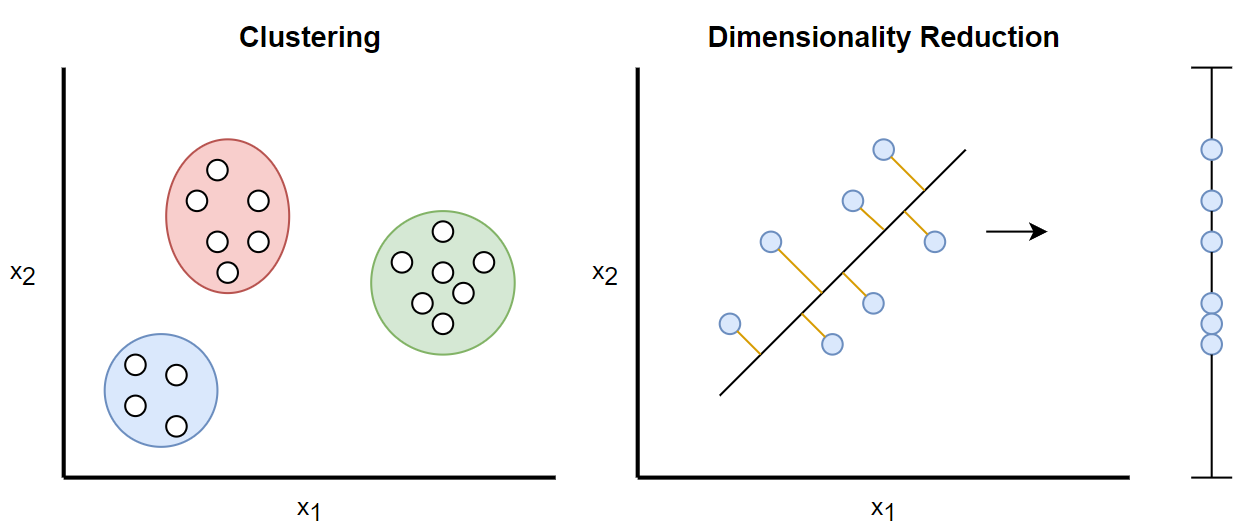
\includegraphics[width=0.8\linewidth]{clustering_vs_DR.png}
        \caption{Clustering vs Dimensionality Reduction. Adapted from~\cite{Beck2020AModelling}}
        \label{fig:clustering_vs_DR}
    \end{figure}

In unsupervised \gls{ML}, several algorithms and computing approaches are utilized. The following are some of the most popular clustering and dimensionality reduction algorithms: K-means clustering and \gls{PCA}~\cite{Chugh2018TypesKnow}.

K-means clustering is a clustering \gls{ML} technique in which data points are divided into \textit{K} groups. The data points nearest to a certain centroid will be clustered together. Smaller groupings with more granularity are indicated by a higher \textit{K} value, whereas bigger groupings with less granularity are indicated by a lower \textit{K} value~\cite{2020WhatIBMb}. Figure~\ref{fig:k_means} provides a visual representation of K-means clustering, with \textit{K} = 3. 
    
\begin{figure}[htbp]
    \centering
    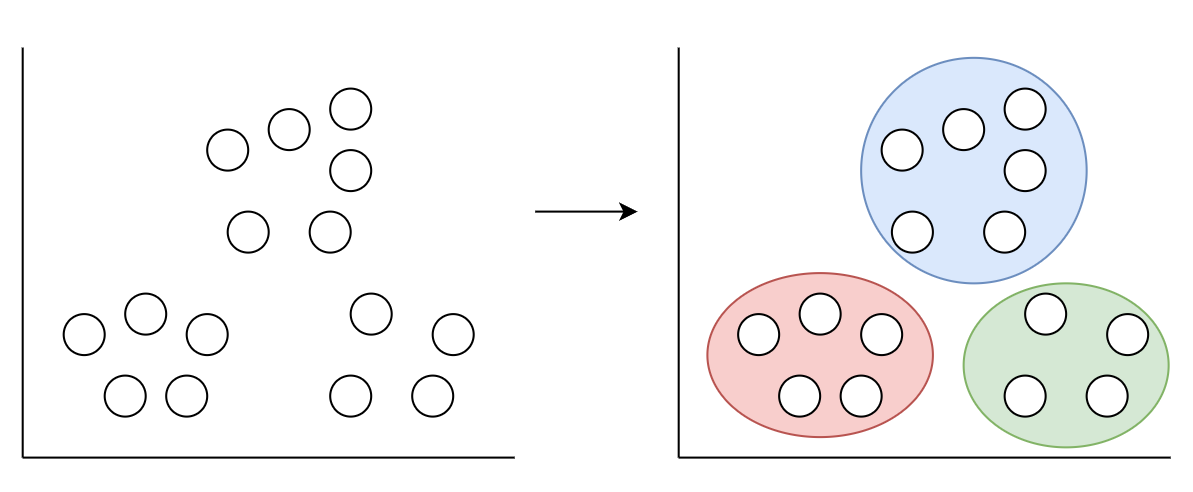
\includegraphics[width=0.65\linewidth]{k-means.png}
    \caption{Visual representation of K-means clustering. Adapted from~\cite{Beaumont2020ImageMedium}}
    \label{fig:k_means}
\end{figure}

\gls{PCA} is a dimensionality reduction approach that uses feature extraction to eliminate redundancies and compress datasets, while retaining as much of the information contained in the original data as possible~\cite{2020WhatIBMb}. Working with too many variables can be difficult for \gls{ML} since there is a chance of overfitting, a lack of appropriate data for each variable, and a degree of correlation between each variable and the output~\cite{Chugh2018TypesKnow}. \gls{PCA} does this by projecting data onto a lower-dimensional subspace that preserves the majority of the variance between data points. Figure~\ref{fig:pca} depicts an example of \gls{PCA}'s influence on 2-dimensional space data.

\begin{figure}[htbp]
    \centering
    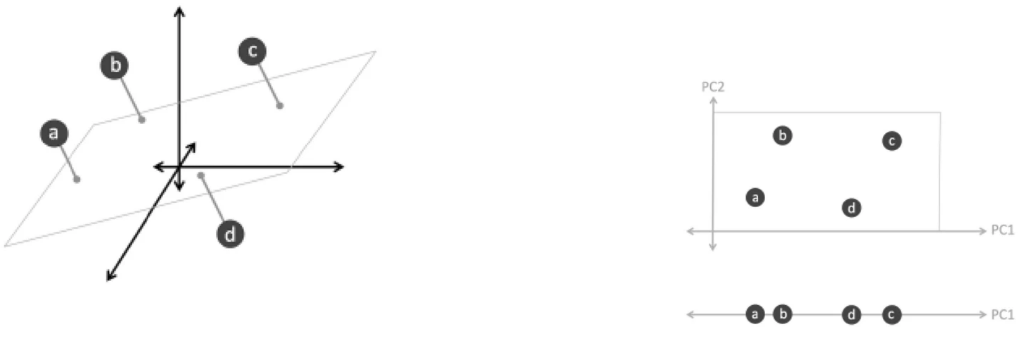
\includegraphics[width=0.5\linewidth]{pca.png}
    \caption{Principal Component Analysis application on 2D space data. Adapted from~\cite{Patcher2014WhatDNA}}
    \label{fig:pca}
\end{figure}

The green line was created through mathematical optimization in order to maximize the variance between the data points as much as possible along that line. This line is referred to as the first principal component. Since a dimension has been lost to separate them, the points on the line are closer to each other than they were in the original 2D environment. However, in many circumstances, the simplification in dimensionality compensates the loss of information. When moving to higher dimensions, it will most likely be necessary to use multiple principal components since the variance described by one principle component will not be enough. Principal components are vectors that form a 90-degree angle between each other (orthogonal vectors), and are independent in a way that the second principal component does not overlap with the variance explained by the first. The first principal component will capture the majority of the variance; the second will catch the second-largest portion of the variance left unexplained by the first, and so on.

\section{Supervised learning}

Supervised learning is a \gls{ML} paradigm for obtaining knowledge about a system's input-output relationship from a set of paired input-output training examples~\cite{Liu2012SupervisedLearning}, with classification and regression being the two most common supervised categories. In classification, a class label is predicted for a given sample. In other words, it maps a function from input variables to output variables as target, label or categories~\cite{Sarker2021MachineDirections}.
In addition, there are multiple classification problems, such as binary classification, which refers to tasks with two class labels, such as "true and false", multiclass classification, which refers to classification tasks having more than two class labels, and multi-label classification when an example is associated with multiple classes or labels. On the other hand, regression contains approaches for predicting a continuous output variable based on the value of one or more predictor variables. The most important difference between classification and regression is that classification predicts distinct class labels, whereas regression predicts a continuous quantity. A clearer distinction between classification and regression is illustrated in Figure~\ref{fig:regression_vs_classification}.
    
\begin{figure}[htbp]
    \centering
    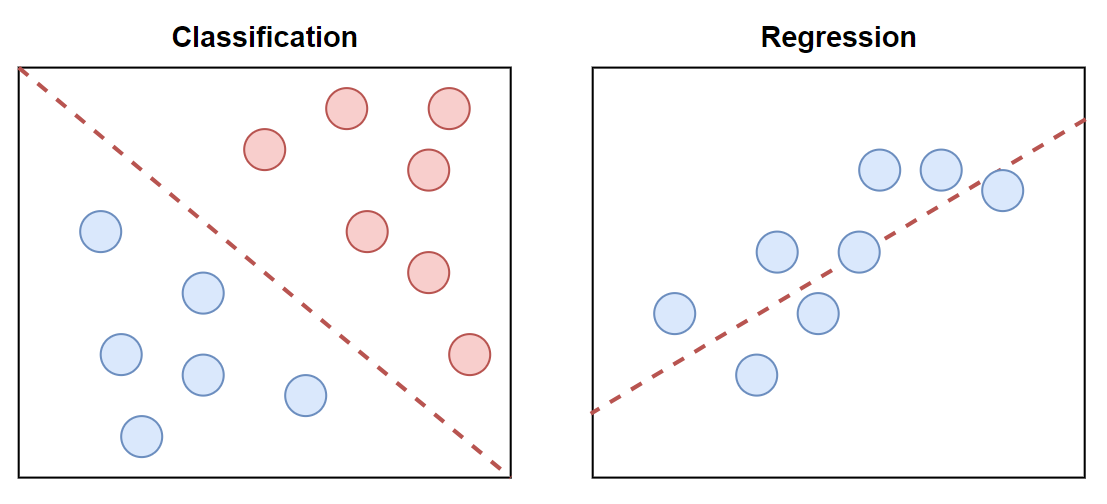
\includegraphics[width=0.75\linewidth]{regression-vs-classification.png}
    \caption{Classification vs Regression. Adapted from~\cite{Matanga2017AnalysisInterfaces}}
    \label{fig:regression_vs_classification}
\end{figure}


While there are several supervised learning algorithms available, most of them follow the same fundamental steps for producing a predictor model. The next section describes the general workflow process of building a supervised machine learning project.

\subsection{Workflow}\label{sec:workflow}

\gls{ML} workflows specify which phases of a \gls{ML} project are implemented. While these measures are widely acknowledged as best practices, there is still potential for improvement. 

When developing a \gls{ML} workflow, the first step is to define the project before determining the best working strategy or attempting to fit the model into a predetermined workflow. Instead, a flexible workflow should be created to start small and work its way up to a production-ready solution.

The steps taken during a \gls{ML} implementation are defined by workflows. \gls{ML} workflows differ depending on the project, but they usually consist of seven steps.

\begin{enumerate}
    \item \textbf{Data Gathering} It is the practice of acquiring and analyzing data from a variety of sources. Data must be collected and kept in a form that makes sense for the challenge at hand in order to be used to build a viable machine learning model. This phase is crucial because the quality and quantity of data collected will directly affect how accurate the predictive model is. Publicly available datasets are frequently the best source of data, and websites like \textit{Kaggle} provide an enormous quantity of huge datasets. Working with these selected datasets reduces the time and effort required to begin a \gls{ML} project.
    
    Structured, semi-structured, and unstructured data are examples of different types of data, and Table~\ref{tab:data_types} provides details about each one of them.
    
    \begin{table}[ht]
    	\caption{Types of data. Adapted from~\cite{Sarker2021MachineDirections}}
        \label{tab:data_types}
    \centering
    \begin{tabular}{p{2.5cm}cc}
    	\toprule
    	\multicolumn{1}{c}{\textbf{Data type}} & \textbf{Description} & \textbf{Examples} \\
    	\midrule
    	
        Structured
        & 
        \begin{tabular}[c]{@{}c@{}}
            Well-defined structure, well-organized\\
            and accessible. Often stored in a tabular\\
            manner such as relational databases.
        \end{tabular} 
        &
        \begin{tabular}[c]{@{}c@{}}
            names, addresses,\\
            credit card numbers
        \end{tabular}
        \\\midrule
        
        Unstructured
        & 
        \begin{tabular}[c]{@{}c@{}}
            Since there is no pre-defined format or\\
            organization, it is significantly more\\
            difficult to acquire, handle, and analyze\\
            data that is largely text and multimedia.
        \end{tabular} 
        &
        \begin{tabular}[c]{@{}c@{}}
            emails, PDF files,\\
            audio files,\\
            videos, photos
        \end{tabular}
        \\\midrule
        
        Semi-structured
        & 
        \begin{tabular}[c]{@{}c@{}}
            Contains organizational qualities that\\
            make it easier to examine.
        \end{tabular} 
        &
        \begin{tabular}[c]{@{}c@{}}
            HTML, XML,\\
            JSON documents
        \end{tabular}
        \\
        
    	\bottomrule
    \end{tabular}
    \end{table}
    
    \item \textbf{Data pre-processing} Cleaning, validating, and converting data into a usable dataset, are all part of pre-processing. This may be a simple operation if the data was collected from a single source. If not, the data format must match between the different sources and be equally credible without any potential duplicates. The majority of real-world data is disorganized; examples include:
    \begin{itemize}
        \item \textbf{Missing data}: when it is not created continuously or when there are technical issues with the application.
        \item \textbf{Noisy data}: also known as outliers, this can be caused by human error (manually obtaining data) or a technical issue with the device at the time of data collection.
        \item \textbf{Inconsistent data}: This type of data may be gathered as a result of human error (mistakes in names or values) or data duplication.
    \end{itemize}
    
    And there are types of raw data too, including:
    
    \begin{itemize}
        \item \textbf{Numeric}: height, weight, age, IQ.
        \item \textbf{Categorical}: race, sex, nationality.
        \item \textbf{Ordinal}: low/medium/high, education level ("high school", "BS", "MS", "PhD").
    \end{itemize}
    
    However, there is an important aspect of \gls{ML} models as they can only handle numeric features. As a result, all types of data must be converted into numeric features. This process of transforming raw data, such as images or text, into suitable modelling features is called feature extraction.
    
    Most of the time, datasets have an excessive number of features that are not required for the predictive model. In fact, removing irrelevant features and keeping the sufficient and essential ones can help reduce the \gls{ML} model training time, as well as reduce overfit and improve accuracy. This filtering process is called feature selection and is usually performed after feature extraction.
    
    \item \textbf{Splitting the Data} It is usual to divide a dataset into two portions for creating \gls{ML} models: training and testing. The training set is used to estimate the model's parameters. The accuracy of the model is then tested using the test dataset. This dataset splitting process is done to prevent overfitting. If the entire dataset was used for training, then the model would overfit the data, meaning it would fail to generate accurate predictions on unseen data~\cite{Joseph2020SPlit:Splitting}.
    
    The simplest and most popular approach for dividing such a dataset is to randomly sample a portion of it. For example, 80\% of the dataset's rows can be randomly selected for training, while the remaining 20\% can be utilized for testing~\cite{Joseph2020SPlit:Splitting}.
    
    It's also typical to save a part of the training set for validation purposes. The validation set may be used to fine-tune the model's performance by selecting hyper-parameters (constant parameter whose value is determined before the learning process) and regularization parameters~\cite{Joseph2020SPlit:Splitting}.
    
    \item \textbf{Building the model} The key goal now is to choose the type of model which fits better the desired problem.
    
    Data can be any of the types listed above (Table~\ref{tab:data_types}), and they can differ from one application to the next in the real world. Therefore, different types of \gls{ML} approaches can be used to evaluate a specific problem field and extract insights or usable knowledge from the data to construct real-world intelligent systems.
    One of the models described in Section~\ref{sec:models_and_algo} that best suits the problem's goal should be chosen.
    
    \item \textbf{Training and evaluation} The objective now is to use the pre-processed data to train the best-performing chosen model, followed by its performance evaluation. 
    The training set will be used to train the model and then the model outputs will be compared with the unseen values. To evaluate these outputs, multiple metrics are used which can vary depending on the problem. 
    
    For binary classification problems, the most commonly metrics include: confusion matrices, accuracy, recall, precision and f1-score~\cite{Liu2014AEvaluation}. These are based on \gls{TP}, \gls{TN}, \gls{FP} and \gls{FN} values, which are the four possible predictions outcomes for a classification problem. \gls{TP} outcomes are correct predictions of the positive class, while \gls{TN} still are correct predictions but of the negative class. \gls{FP} outcomes are incorrect predictions of the positive class, while \gls{FN} still are incorrect predictions but of the negative class. 
    
    The confusion matrices are tables which rows represent the real classes and the columns represent the predicted classes. So, for each class, the table shows how many predictions were and were not correct. Figure~\ref{fig:conf_matrix} shows an example of a confusion matrix and Figure~\ref{fig:conf_matrix2} illustrates how the the \gls{TP}, \gls{TN}, \gls{FP} and \gls{FN} values are perceived within the table.
    
    \begin{figure}[htbp]
        \centering
        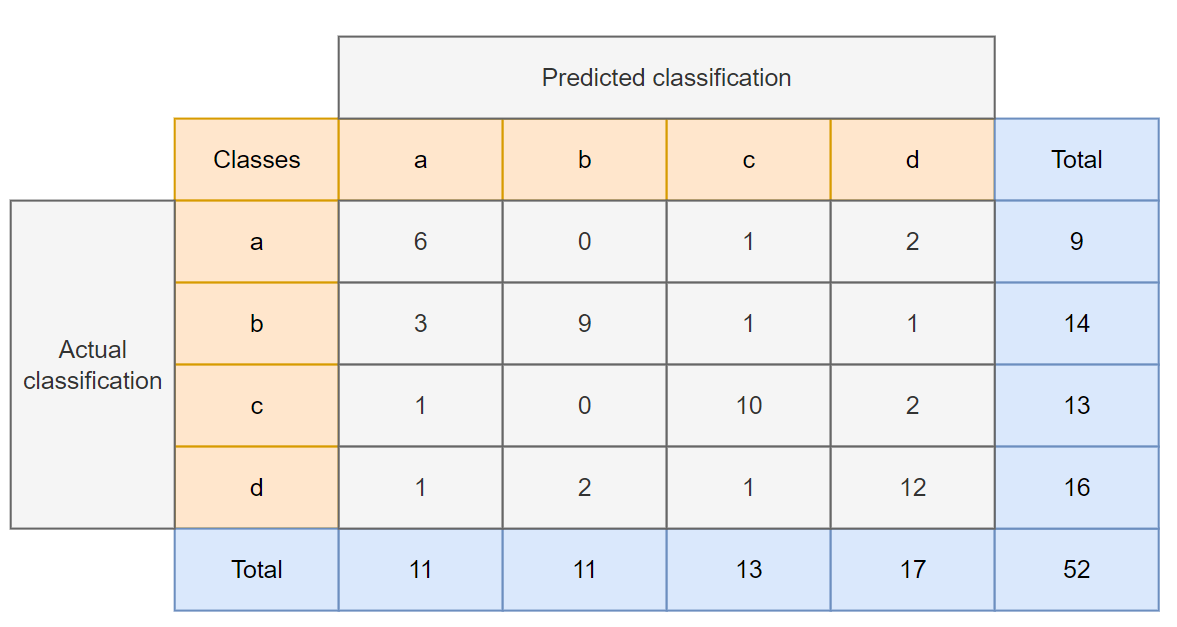
\includegraphics[width=0.7\linewidth]{conf_matrix.png}
        \caption{Example of confusion matrix}
        \label{fig:conf_matrix}
    \end{figure}
    
    \begin{figure}[htbp]
        \centering
        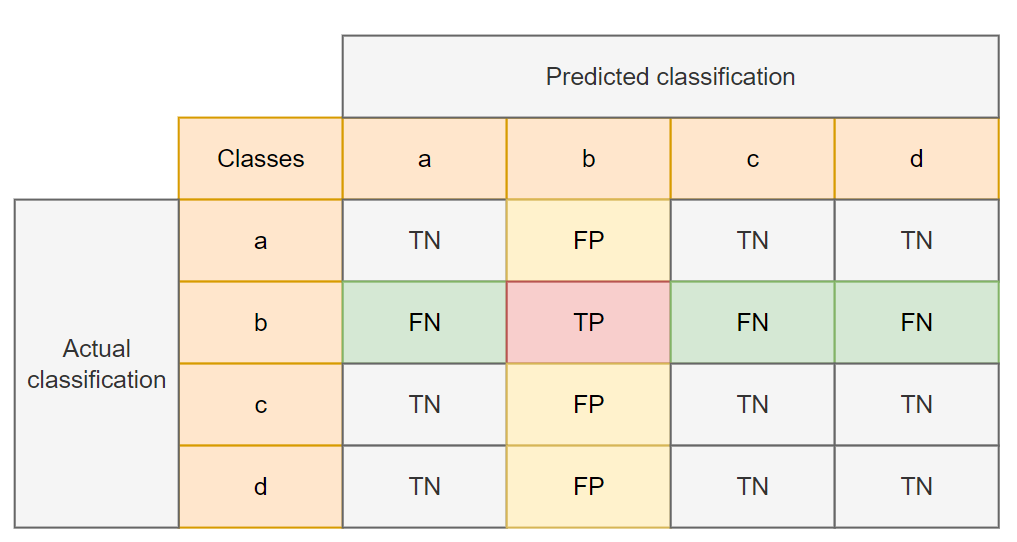
\includegraphics[width=0.65\linewidth]{conf_matrix2.png}
        \caption{Example of confusion matrix with the prediction outcomes, relative to the \textit{b} class}
        \label{fig:conf_matrix2}
    \end{figure}
    
    After defining \gls{TP}, \gls{TN}, \gls{FP} and \gls{FN} values, the other classification metrics are simple to calculate. Table~\ref{tab:classification_metrics} explains each classification metric and how each one is calculated.
    
    \begin{table}[ht]
    	\caption{Classification evaluation metrics}
        \label{tab:classification_metrics}
    \centering
    \begin{tabular}{p{2.5cm}cc}
    	\toprule
    	\multicolumn{1}{c}{\textbf{Metric}} & \textbf{Description} & \textbf{Equation} \\
    	\midrule
    	
        Accuracy
        & 
        \begin{tabular}[c]{@{}c@{}}
            Fraction of correct predictions. 
        \end{tabular} 
        &
        \begin{tabular}[c]{@{}c@{}}
            \(\displaystyle \frac{TP + TN}{TP + TN + FP + FN} \)
        \end{tabular}
        \\\midrule
        
        Recall
        & 
        \begin{tabular}[c]{@{}c@{}}
            Proportion of actual positives correctly identified
        \end{tabular} 
        &
        \begin{tabular}[c]{@{}c@{}}
            \(\displaystyle \frac{TP}{TP + FN} \)
        \end{tabular}
        \\\midrule
        
        Precision
        & 
        \begin{tabular}[c]{@{}c@{}}
            Proportion of positive identifications actually correct
        \end{tabular} 
        &
        \begin{tabular}[c]{@{}c@{}}
            \(\displaystyle \frac{TP}{TP + FP} \)
        \end{tabular}
        \\\midrule
        
        F1-score
        & 
        \begin{tabular}[c]{@{}c@{}}
            Harmonic mean between precision and recall.
        \end{tabular} 
        &
        \begin{tabular}[c]{@{}c@{}}
            \(\displaystyle 2\times\frac{precision \times recall}{precision + recall} \)
        \end{tabular}
        \\
        
    	\bottomrule
    \end{tabular}
    \end{table}
    
    For regression problems, the most commonly metrics include: \gls{MSE}, \gls{MAE} and \gls{MAPE}~\cite{Botchkarev2018PerformanceTypology}. They are calculated using the difference between the predicted and the actual value. \gls{MSE} measures the average squared difference between the predicted values and the real value. Over all occurrences in the test set, \gls{MAE} determines the mean of the absolute values of the individual prediction errors and \gls{MAPE} determines the mean of the absolute percentage errors of the individual prediction errors. 
    
    Since the objective is to build a model that can generalize the information on unseen data, it is also important to measure the generalization performance of the model. This can be achieved by applying the k-fold cross-validation method, which uses \textit{k} different partitions of the dataset to train and test a model on different iterations. Of the \textit{k} portions, \textit{k-1} portions are used as training data and the remaining portion is the validation data to test the model. This process is repeated until all partitions are tested, meaning it has \textit{k} iterations until it ends.
    
    \item \textbf{Hyperparameter Tuning} It is the process of selecting a set of ideal hyperparameters for a learning algorithm. A hyperparameter is a model parameter whose value is determined prior to the start of the learning process, since it cannot be learned during the training process.
    
    \item \textbf{Prediction} After obtaining an acceptable performance, guided by the evaluation phase, the next and final step is to put the developed model to work. After all this effort, the benefit of \gls{ML} is recognized at this step. The benefit of \gls{ML} is that it enables one to obtain an accurate prediction by feeding input data to the model rather than relying on human judgment and manual rules.

\end{enumerate}

\subsection{Models and algorithms}\label{sec:models_and_algo}

In supervised \gls{ML}, several algorithms and computing approaches are utilized. The following are some of the most popular classification and regression algorithms: \gls{LR}, \gls{LgR}, \gls{KNN}, \gls{SVM}, \gls{DT}, \gls{RF} and \gls{ANN}~\cite{2020WhatIBM,Chugh2018TypesKnow}.

% Linear Regression
\gls{LR} is the most popular method of regression analysis, which assumes that the dependent variable (variable to be predicted) and the independent variable (base for the variable to be predicted) have a linear relationship. Linear regression creates a model for the best fit line between two variables. The outcome of interest must be a continuous variable in order to be appropriate for \gls{LR}~\cite{Worster2007UnderstandingAnalyses}. Figure~\ref{fig:linear_regression} shows how the model (red line) is created by utilizing training data (blue points) with known labels (y axis) to fit the points as exactly as possible by minimizing the value of a given loss function (usually \gls{MSE}).

\begin{figure}[htbp]
    \centering
    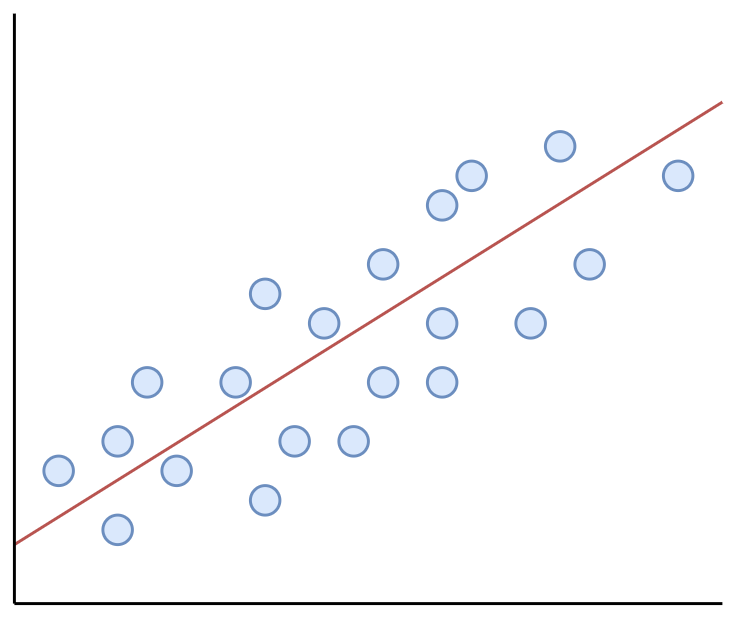
\includegraphics[width=0.4\linewidth]{linear_regression.png}
    \caption{Visual representation of Linear Regression. Adapted from~\cite{Nasteski2017AnMethods}}
    \label{fig:linear_regression}
\end{figure}

% Logistic Regression
\gls{LgR} is similar to \gls{LR} but it is used for classification problems. To model a binary output variable, logistic regression employs the logistic function given below (Eq~\ref{eq:5}). The main distinction between linear and logistic regression is that the range of logistic regression is limited to 0 and 1. Furthermore, logistic regression does not require a linear connection between input and output variables, unlike linear regression. Also unlike linear regression, which employs \gls{MSE} as the loss function, logistic regression utilizes a conditional probability loss function called \gls{MLE}. The predictions will be categorized as class 0 if the probability is larger than 0.5. Otherwise, you will be allocated to class 1~\cite{Belyadi2021SupervisedLearning}. By default, logistic regression cannot be utilized for multi-class classification problems, which have more than two class labels. However, it is possible to adapt logistic regression to solve  multi-class classification problems. One approach example is to divide the multi-class classification issue into several binary classification problems and apply a typical logistic regression model to each subproblem. 

\begin{equation}\label{eq:5}
    f(x) = \frac{1}{1+e^{-x}}
\end{equation}


% KNN
The \gls{KNN} algorithm is a classification/regression technique that classifies data points based on their proximity and correlation with other data~\cite{2020WhatIBM}. This technique assumes that data points that are comparable can be located close together. As a result, it attempts to determine the distance between data points, which is commonly done using Euclidean distance, and then assigns a category based on the most common category or average. Depending on the value of \textit{K} (the number of nearest neighbors that will participate in the voting process), different results can be obtained. In Figure~\ref{fig:knn}, the test sample (green circle) should fall into one of two categories: squares or triangles. If \textit{K} = 3, then only the three nearest neighbors to the test sample will participate in the voting process. In this example, it is assigned to the triangles class since the nearest neighbors are two triangles and only one square. If \textit{K} = 5, it is assigned to the squares class because the five nearest neighbors are three squares and only two triangles.

\begin{figure}[htbp]
    \centering
    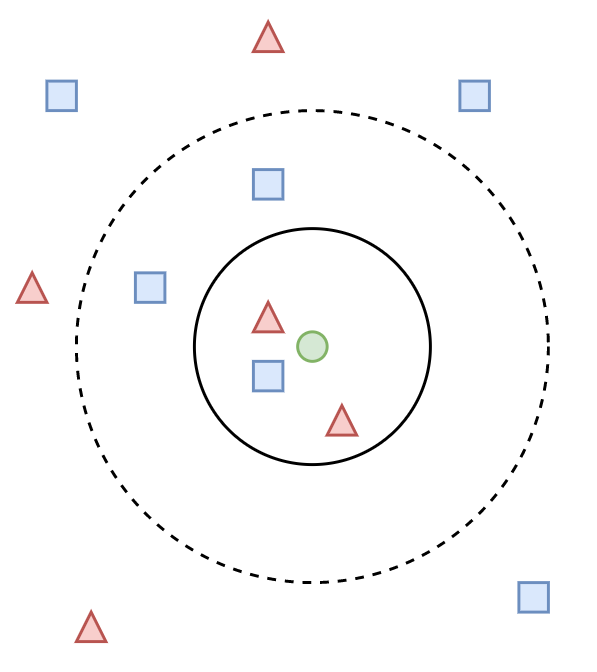
\includegraphics[width=0.4\linewidth]{knn.png}
    \caption{Visual representation of K-Nearest Neighbors. Adapted from~\cite{Bronshtein2017AMedium}}
    \label{fig:knn}
\end{figure}

% SVM
\gls{SVM}s are supervised learning models that evaluate data for classification and regression analysis. They create hyperplanes that are drawn at the maximum distance between two classes from the training data points (support vectors), since the greater the margin, the lower the classifier's generalization error. Then, new samples are predicted to belong to a category according to which side of the gap they fall~\cite{Mahesh2019MachineReview}. Figure~\ref{fig:svm} provides an example of a linear classification perfomed by \gls{SVM}. If a new sample fell to the right of the hyperplane, it would be classified as the red dot class, and it would otherwise be classified as the blue dot class if it fell to the left of the hyperplane. 

\begin{figure}[htbp]
    \centering
    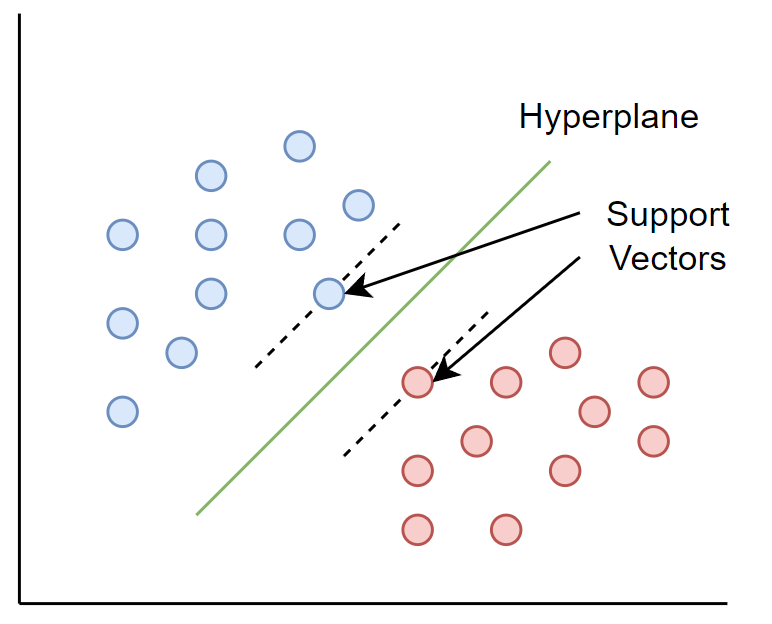
\includegraphics[width=0.5\linewidth]{svm.png}
    \caption{Visual representation of Support Vector Machines. Adapted from~\cite{MaquinaExplicada}}
    \label{fig:svm}
\end{figure}

However, with the help of kernel functions, \gls{SVM}s may do non-linear classification as well by implicitly translating their inputs into high-dimensional feature spaces. Some examples of kernel functions used in \gls{SVM} classifiers are linear, polynomial and radial basis functions.

% Decision tree
\gls{DT} learning is a supervised \gls{ML} technique for producing a decision tree from training data. \gls{DT} builds classification or regression models in the form of a tree structure. It is a model that consists of a mapping from item observations to conclusions about its target value. In tree structures, leaves indicate labels, nonleaf nodes represent features, and branches represent combinations of features that lead to decisions on the target~\cite{Tan2015CodeQuality}.

\begin{figure}[htbp]
    \centering
    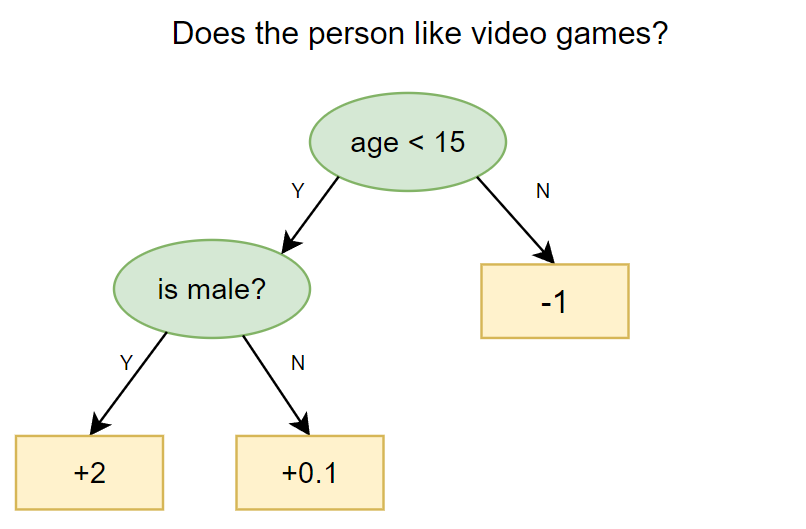
\includegraphics[width=0.6\linewidth]{dt.png}
    \caption{Visual representation of Decision Tree}
    \label{fig:dt}
\end{figure}

% Random forest
A \gls{RF} classifier is an ensemble \gls{ML} algorithm. One note should be added regarding ensemble methods before addressing \gls{RF}. Ensemble learning is the process of building and combining many models to tackle a specific computational issue. Ensemble learning is generally used to improve a model's performance or reduce the risk of an unintentionally poor model selection~\cite{Mahesh2019MachineReview}. Bagging is an ensemble learning technique for reducing variance in a noisy dataset. It consists of selecting a random sample of data from a training set with replacement (individual data points might be used multiple times). These weak models are then trained individually after multiple data samples are collected, and depending on the kind of task (for example, regression or classification), the average or majority of those predictions provides a more accurate estimate. Knowing this, \gls{RF} employs parallel ensembling, in which numerous \gls{DT} classifiers are fitted in parallel on distinct dataset sub-samples, as illustrated in Figure~\ref{fig:random_forest2}, and the final result is determined by majority voting or averages. Therefore, the overfitting problem is reduced, and prediction accuracy and control are improved. As a result, a \gls{RF} learning model based on many \gls{DT}s is usually more accurate than one based on a single \gls{DT}. It combines the previously mentioned bagging technique with random feature selection to create a succession of \gls{DT}s with controlled variance. It works well for both categorical and continuous variables and may be applied to both classification and regression issues~\cite{Sarker2021MachineDirections}.

\begin{figure}[htbp]
    \centering
    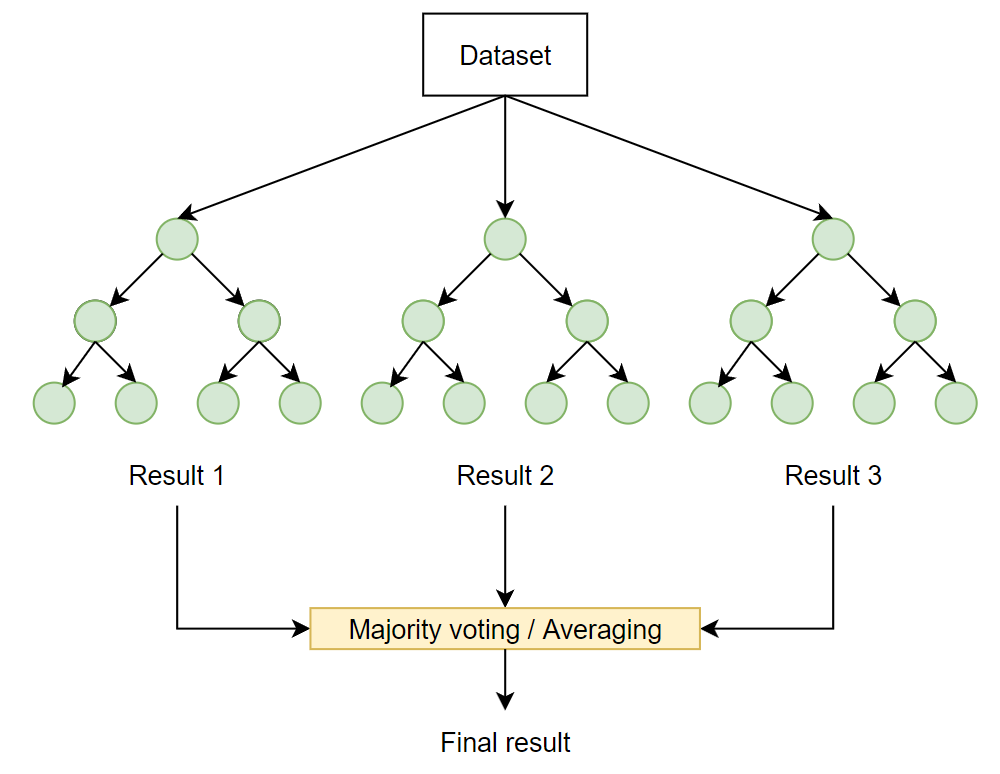
\includegraphics[width=0.65\linewidth]{rf.png}
    \caption{Random Forest structure. Adapted from~\cite{Sarker2021MachineDirections}}
    \label{fig:random_forest2}
\end{figure}

% ANN
\gls{ANN}s-based supervised classifiers are extremely sophisticated and may be further subdivided into a number of distinct but related ideas. They are based on the neural network of the brain. These algorithms are used in most cutting-edge artificial intelligence applications and are typically used when working with very big datasets. They also serve as the foundation for deep learning approaches, as detailed below in both sections~\ref{sec:ann} and ~\ref{sec:dl}.

\subsection{Artificial neural networks}\label{sec:ann}

In general, a biological neuron accepts inputs and arranges them to perform an operation, which results in the final output. When looking at biological neurons, there are four major components: dendrites, cell bodies, axons, and synapses. Dendrites are in charge of accepting incoming impulses into the cell body. The cell body subsequently processes these electrical signals and converts them to the final output. The output signal is then transferred from the cell body to the other neurons through the axon, which serves as a transmission line between neurons. Synapses are the locations placed between neurons and dendrites that are responsible for gathering input from neurons~\cite{Imran2019AClassification}. 

\gls{ANN} is a supervised \gls{ML} algorithm that is inspired by the biological structure and function of the human brain and, as seen in Figure~\ref{fig:an}, the intricacy of biological neurons in the brain can be mimicked.

\begin{figure}[htbp]
    \centering
    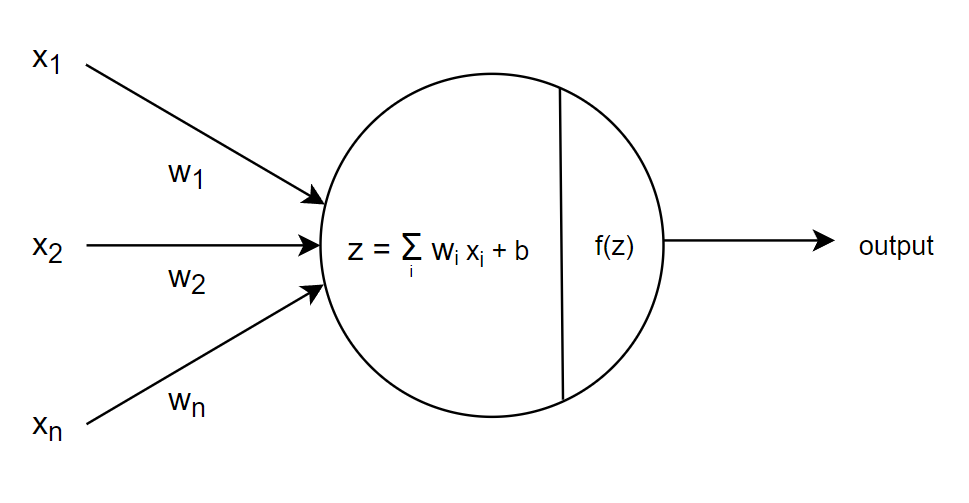
\includegraphics[width=0.75\linewidth]{an.png}
    \caption{Artificial neuron. Adapted from~\cite{Baheti12Choose}}
    \label{fig:an}
\end{figure}

In the case of \gls{ANN}, inputs are directed to the body of an artificial neuron. In Figure~\ref{fig:an}, X(n) represents the inputs; each input is multiplied by its associated weight, which is a measure of the input's connection strength and is represented by W(n). The summing function is then given weighted inputs and the bias (b). The summing function's value (z) will be sent to the activation function (f), which will yield the final output~\cite{Imran2019AClassification}. Activation functions specify a range of values for the neuron's output, determining if the neuron's input to the network is essential or not~\cite{2020ArtificialNetworks}. Some examples of activation functions are sigmoid (Eq~\ref{eq:1}), TanH (Eq~\ref{eq:2}), and ReLU (Eq~\ref{eq:3})~\cite{EnyinnaNwankpa2018ActivationLearning}.

%%%%%%%%%%%%%%%%%%%%%%%%%%%%%%%%%%%%%%%%%%%%%%%%%%%%%%%%%%%%%%%%%%%%%%%%%%%%%%%%%%%%%%%%%%%%

\begin{equation}\label{eq:1}
    f(x) = \frac{1}{1+e^{-x}}
\end{equation}

\begin{equation}\label{eq:2}
    f(x) = \frac{e^{x}-e^{-x}}{e^{x}+e^{-x}}
\end{equation}

\begin{equation} \label{eq:3}
    f(x) = \begin{cases}x & x \geq 0\\0 & x < 0\end{cases}
\end{equation}

The weights of an \gls{ANN} are initially randomly assigned, but they are updated during the training process. This is possible by applying both forward and back propagation. In forward propagation, information travels in one direction only: forward. Inputs are fed into the neural network, and the produced outputs are compared to the real ones, with a loss function used to determine the difference~\cite{Farizawani2020AApproaches}. Then, in back propagation, the internal weights are adjusted using optimization methods to reduce the loss function~\cite{Kim2021CBP:Method}. 

An \gls{ANN} is composed of three layers: an input layer, a hidden layer, and an output layer. There must be a link between the nodes in the input layer and the nodes in the hidden layer, as well as between each node in the hidden layer and the nodes in the output layer~\cite{Imran2019AClassification}. In the input layer, each neuron represents an input feature, and no computation is performed. In the hidden layer the nodes are not visible. They serve as an abstraction for the neural network. The hidden layer performs all types of calculations on the features received through the input layer by using a weighted linear summation followed by an activation function, and sends the results to the output layer. Then the output layer takes the information learnt from the hidden layer and provides the final value. The number of output neurons represents the number of predictions. This means that, if it is a regression or binary classification problem, this layer will only have one neuron. If it is a multiclass classification problem, the number of neurons will be equal to the number of classes~\cite{Alaloul2020DataNetworks}. Figure~\ref{fig:ann} shows an example of an \gls{ANN}'s structure.

\begin{figure}[htbp]
    \centering
    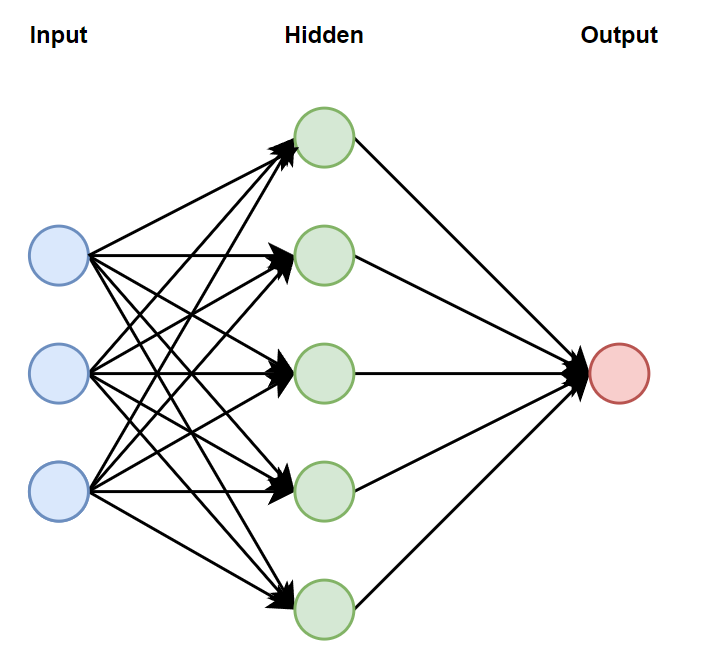
\includegraphics[width=0.55\linewidth]{ann.png}
    \caption{Artificial Neural Network}
    \label{fig:ann}
\end{figure}

\section{Deep Learning}\label{sec:dl}

\gls{DL} is a subset of \gls{ML} whose methods are based on multi-layered \gls{ANN}s with feature learning techniques. These techniques enable a system to automatically identify the representations required for feature detection from raw data. This eliminates the need for human feature engineering by allowing a machine to learn the features and then use them to execute a specified activity. But, for this to be possible, \gls{DL} algorithms demand larger amounts of data.

The simplest \gls{DL} architecture is the \gls{DNN}. A \gls{DNN} is an \gls{ANN} with various layers between the input layer and the output layers. In other words, a \gls{DNN} has multiple hidden layers~\cite{Schmidhuber2015DeepOverview}. Figure~\ref{fig:ann-vs-dnn} shows a visual distinction between these two architectures.

\begin{figure}[htbp]
    \centering
    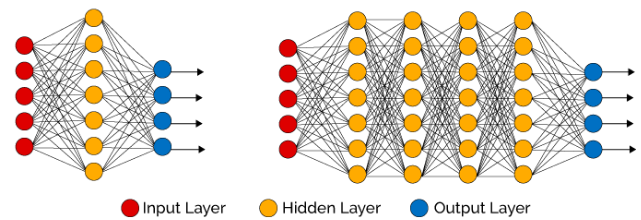
\includegraphics[width=0.8\linewidth]{ann-vs-dnn.png}
    \caption{Artificial Neural Network vs Deep Neural Network}
    \label{fig:ann-vs-dnn}
\end{figure}

The inner workings of the layers and neurons are similar between \gls{ANN} and \gls{DNN}, meaning \gls{DNN}s are feedforward networks that transfer data from the input layer to the output layer without looping back. The \gls{DNN} starts by creating a map of virtual neurons and assigning random weights to their connections. The inputs and weights are multiplied, and the result is a value between 0 and 1. An algorithm would update the weights if the network didn't detect a pattern correctly. As a result, the algorithm might increase the influence of specific factors until it finds the optimal mathematical manipulation to fully analyze the input.

To understand better the concepts of \gls{DL}, Table~\ref{tab:dl_terminologies} provides a few important terminologies.

%%%%%%%%%%%%%%%%%%%%%%%%%%%%%%%%%%%%%%%%%%%%%

\begin{table}[ht]
	\caption{Deep Learning concepts~\cite{MachineDevelopers,Shafkat2018IntuitivelyLearning}}
	\label{tab:dl_terminologies}
\centering
\begin{tabular}{p{0.15\linewidth}c}
	\toprule
	\multicolumn{1}{c}{\textbf{Concept}} & \textbf{Description} \\
	\midrule
	
    Activation Function
    & 
    \begin{tabular}[c]{@{}c@{}}
        Function that takes the weighted sum of all the inputs from\\
		the previous layer and then creates and passes an output value\\
		(usually nonlinear) to the following layer.
    \end{tabular} 
    \\\midrule
    
    Back-propagation
    & 
    \begin{tabular}[c]{@{}c@{}}
        Most commonly used algorithm for Gradient Descent. Begins at the\\
		output layer and traverses the network backwards.
    \end{tabular} 
    \\\midrule
    
    Batch
    & 
    \begin{tabular}[c]{@{}c@{}}
        Set of examples utilized in one model training iteration.
    \end{tabular} 
    \\\midrule
    
    Batch size
    & 
    \begin{tabular}[c]{@{}c@{}}
        The number of examples in a batch. It's an hyperparameter.
    \end{tabular} 
    \\\midrule
    
    Epoch
    & 
    \begin{tabular}[c]{@{}c@{}}
        A full training pass across the entire dataset while updating model\\
		weights. The number of epochs is a key hyperparameter.
    \end{tabular} 
    \\\midrule
    
    Gradient
    & 
    \begin{tabular}[c]{@{}c@{}}
        Vector of partial derivatives with respect to all of the\\
		independent variables.
    \end{tabular} 
    \\\midrule

	Gradient Descent
    & 
    \begin{tabular}[c]{@{}c@{}}
        Technique to minimize loss by computing the gradients of loss with\\
		respect to the model's parameters, conditioned on training data.
    \end{tabular} 
    \\\midrule

	Hyper-parameter
    & 
    \begin{tabular}[c]{@{}c@{}}
        Constant parameter whose value is determined before the\\
        learning process.
    \end{tabular} 
    \\\midrule

	Learning rate
    & 
    \begin{tabular}[c]{@{}c@{}}
        Scalar that is used to train a model with gradient descent. The\\
		gradient descent technique multiplies the learning rate by the\\
		gradient at each iteration, meaning it controls the speed of the\\
		gradient update. It's also a key hyperparameter.
    \end{tabular} 
    \\\midrule

	Loss
    & 
    \begin{tabular}[c]{@{}c@{}}
        Function that calculates the difference between the algorithm's\\
		current output and the expected output.
    \end{tabular} 
    \\\midrule

	Neuron
    & 
    \begin{tabular}[c]{@{}c@{}}
        The neural network's basic unit.
    \end{tabular} 
    \\\midrule

	Optimizer
    & 
    \begin{tabular}[c]{@{}c@{}}
        Specific implementation of the gradient descent algorithm.\\
		Examples are SGD and Adam.
    \end{tabular} 
    \\\midrule

	Parameter
    & 
    \begin{tabular}[c]{@{}c@{}}
        Model variable that is self-taught by the \gls{ML} system. Weights,\\
		for example, are parameters whose values the \gls{ML} system learns\\
		over time through training iterations.
    \end{tabular} 
    \\\midrule
    
    Training
    & 
    \begin{tabular}[c]{@{}c@{}}
        Procedure for determining a model's optimum parameters.
    \end{tabular} 
    \\

	\bottomrule
\end{tabular}
\end{table}

%%%%%%%%%%%%%%%%%%%%%%%%%%%%%%%%%%%%%%%%%%%%%


\subsection{Training phase}

In order to start training a \gls{DL} model, just as \gls{ANN}, the initial model weights are chosen randomly. Then, the model weights are updated to reduce the error between the algorithm's current output and the expected output. This error is measured by the loss function and weight-finding algorithms are used to minimize this function, knows as optimization algorithms. These algorithms are specific implementations of the gradient descent algorithm, which is a technique to minimize loss by computing the gradients of loss with respect to the model's parameters, conditioned on training data. 

Various optimizers are researched within the last few couples of years each having its advantages and disadvantages, but the most commonly used is \gls{SGD}~\cite{Chauhan2020OptimizationNetworks}.

In \gls{SGD}, the back-propagation algorithm is used to compute the gradients of the loss function, and the results are input to the \gls{SGD} method to update the parameters (weights and biases) incrementally after each epoch.

Instead of computing the gradient of the error based on all training samples like GD, \gls{SGD} creates an approximation of the actual gradient error based on a single training sample. As a result of the faster calculation of the approximation, \gls{DNN} can train faster and generalize better with \gls{SGD}~\cite{Amir2021SGDHelp}.

The difference between the non-updated and the updated weight can be controlled using the learning rate hyperparameter and it is possible to define how to calculate the updated weight

\begin{equation}\label{eq:4}
    W_{x}^{'} = W_{x} - a(\frac{\partial Error}{\partial W_{x}})
\end{equation}

where ~$W_{x}^{'}$ is the new weight, ~$W_{x}$ is the old weight, ~$a$ is the learning rate, and ~$\frac{\partial Error}{\partial W_{x}}$ is the gradient (derivative of error with respect to weight)~\cite{Kim2021EasyAlgorithm}. If the value of the learning rate hyperparameter is close to zero, the difference between the old and new weight would be minimal, meaning that the greater the learning rate, the greater the weight differential.

\subsection{Challenges of deep neural networks}

It is difficult to train a \gls{DNN} that can generalize well to unknown input data. A model with insufficient capacity cannot learn the problem, while a model with excessive capacity may learn it too well and overfit the training dataset. In both circumstances, the model does not generalize effectively. However, \gls{DNN}s tend to overfit because of the additional abstraction layers that enable them to model unusual relationships in the training data.

The complexity of a neural network model is determined by both its structure (number of nodes and layers) and its parameters (weights). As a result, in order to reduce overfitting, it is possible to lower a neural network's complexity by changing its structure or its parameters~\cite{Brownlee2019HowNetworks}. Instead of changing the neural network's architecture, it is more typical to limit the model's complexity by changing the model's weights, keeping them as small as possible. Small parameters imply a less complex and, as a result, more stable model that is less susceptible to statistical fluctuations in the input data.

Methods that aim to reduce overfitting by maintaining network weights minimal are referred to as regularization methods and the most common ones include early stopping, L1, L2 and dropout~\cite{Brownlee2019HowNetworks}.

Early stopping takes a straightforward strategy, stopping the network's training when the model does not improve on the validation set score, or, in other words, when the error on the validation set starts to grow.

Weight decay, also known as weight regularization, is another strategy for decreasing overfitting in neural networks. Weight decay penalizes the network for having a high weight distribution by adding a cost to the training loss~\cite{Brownlee2019HowNetworks}. Examples of these methods are L1 and L2. In L1, it applies an L1 penalty equivalent to the absolute value of the magnitude of the coefficient. In L2, It applies an L2 penalty equivalent to the square of the magnitude of the coefficients~\cite{NgFeatureInvariance}.

In dropout, at every iteration of the training process, randomly selected nodes and their connections are dropped from the neural network. This prevents units from over-co-adapting, which would otherwise lead to overfitting problems. The derivative obtained by each parameter in a typical neural network tells it how it should change such that the resultant loss function is minimized, given what the other units are doing. As a result, units may evolve in such a way that they correct the errors of other units, which can lead to complex co-adaptations. This results in overfitting due to the fact that these co-adaptations cannot generalize to unseen data. Dropout makes the presence of additional hidden units unpredictable, preventing co-adaptation. As a result, a hidden unit cannot rely on other units to fix its errors. It must function properly in a wide range of situations created by the other hidden units~\cite{Srivastava2014Dropout:Overfitting}.

In addition to the overfitting problem, \gls{DNN}s also suffer from high computation times. \gls{DNN}s must take into account a variety of training parameters, including the size (number of layers and units per layer), learning rate, and starting weights. Due to the time and processing resources required, sweeping across the parameter space for optimal parameters may not be practical. However, powerful processing hardware such as \gls{GPU}s are ideal for training \gls{DL} models as they can handle numerous computations at the same time. They feature a lot of cores, which makes it easier to run several parallel operations at the same time, resulting in a speed up in the training process.

\subsection{Deep learning architectures}

The growth in the field of \gls{DL} architectures during the last two decades has provided enormous prospects for implementing it in a variety of applications. The next section introduces four popular \gls{DL} architectures: \gls{DNN}, \gls{CNN}, \gls{RNN}, and autoencoders~\cite{Ganatra2018ATools,Madhavan2021DeepDeveloper}.

\paragraph{Deep neural networks} 

As mentioned in Section~\ref{sec:dl}, \gls{DNN}s are feed forward networks, in which data goes from the input layer to the output layer without traveling backwards. They are based on \gls{ANN}s but, unlike them, \gls{DNN}s contain multiple hidden layers. In spite of this, the inner workings of the layers and neurons are similar between \gls{ANN} and \gls{DNN}.

\paragraph{Convolutional neural networks} 

A \gls{CNN} is a multilayer supervised neural network that was originally inspired by the neurobiological process of animal visual cortex~\cite{Ganatra2018ATools}. It is commonly used for processing data with a grid pattern, such as as images and videos. It is built to learn spatial hierarchies of features automatically, from low-level to high-level patterns. 

\gls{CNN}s are made up of three types of layers: convolutional, pooling, and fully connected layers. In general, the convolutional layer extracts features from the input, the pooling layer minimizes the size of the input data to the following layers, and the fully connected layers map the features into a final output, such as classification. Figure~\ref{fig:cnn} provides an overview of the architecture of a \gls{CNN} and how it is trained. The performance of a model with certain kernels and weights is determined using a loss function and forward propagation and they are updated using the gradient descent optimization process.

\begin{figure}[htbp]
    \centering
    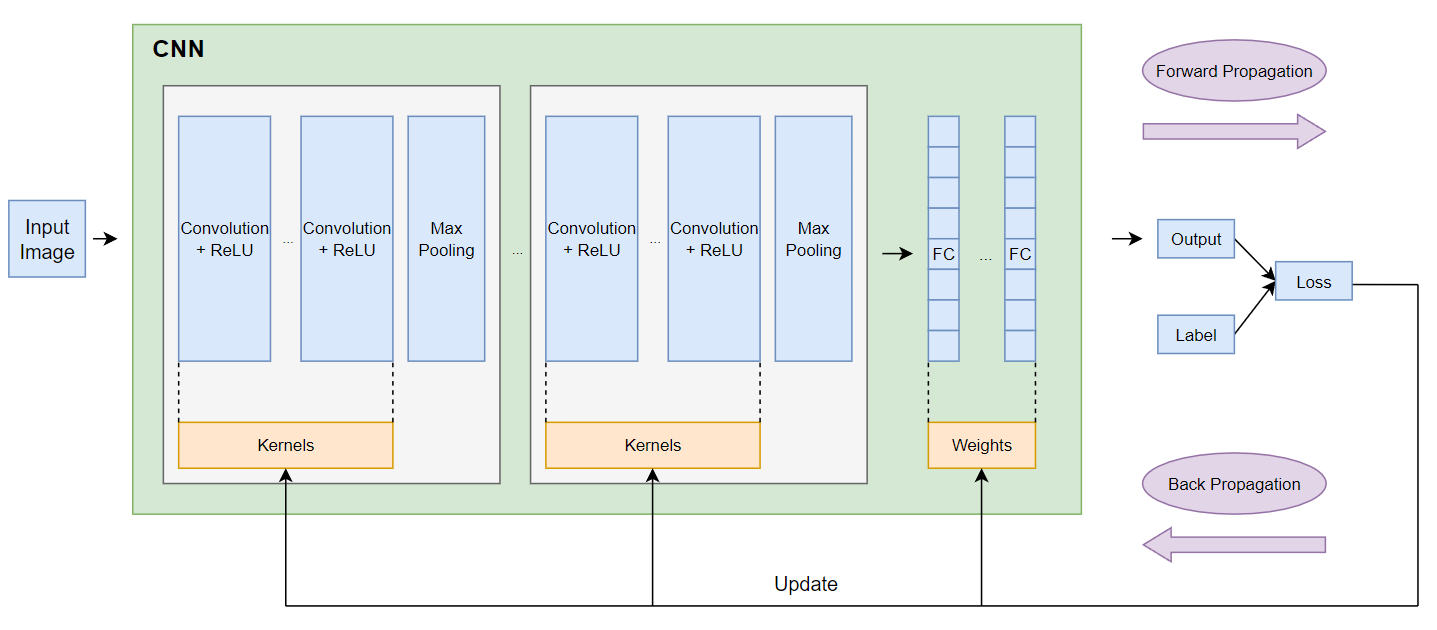
\includegraphics[width=\linewidth]{cnn.png}
    \caption{Convolutional Neural Network architecture. Adapted from~\cite{Yamashita2018ConvolutionalRadiology}}
    \label{fig:cnn}
\end{figure}

% Convolutional layer
The convolutional layer is a key component of the \gls{CNN} architecture that conducts feature extraction using a mix of linear and nonlinear techniques, such as convolution and activation functions. Convolution is a form of linear operation used for feature extraction in which a tiny array of numbers, called a kernel, is applied over the tensor, which is also an array of numbers. At each point of the tensor, an element-wise product between each element of the kernel and the input tensor is computed and added to generate the output value in the corresponding place of the output tensor, referred to as a feature map (Figure~\ref{fig:merge_cnn}). This technique is done with several kernels to create an arbitrary number of feature maps that reflect distinct features of the input tensors; hence, different kernels may be regarded as different feature extractors. The size and number of kernels are two fundamental hyperparameters that determine the convolution operation~\cite{Yamashita2018ConvolutionalRadiology}.

\begin{figure}[htbp]
    \centering
    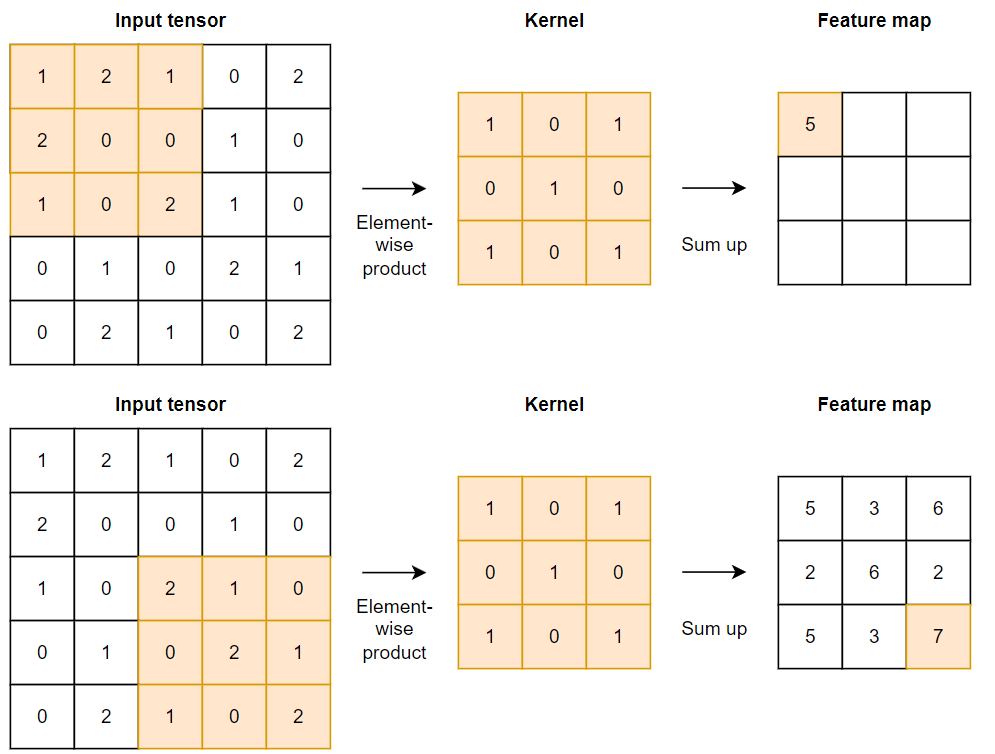
\includegraphics[width=0.85\linewidth]{merge_cnn.png}
    \caption{Convolution operation with a kernel size of 3 × 3, no padding, and a stride of 1. Adapted from~\cite{Yamashita2018ConvolutionalRadiology}}
    \label{fig:merge_cnn}
\end{figure}

The stride is the distance between two consecutive kernel points, and a stride of 1 is the most popular choice. However, a stride greater than 1 is occasionally used to accomplish feature map downsampling. The pooling procedure is the alternate approach for downsampling.

It is important to emphasize that the above convolution method prevents the center of each kernel from overlapping the input tensor's outermost element, thereby reducing the output feature map's height and width in comparison to the input tensor. Padding, usually zero padding, is a strategy for dealing with this problem that involves adding rows and columns of zeros on either side of the input tensor in order to fit the center of a kernel on the outermost element while maintaining the same in-plane dimension during the convolution process. After the convolution procedure, each subsequent feature map would be smaller if there was no padding~\cite{Yamashita2018ConvolutionalRadiology}.

Identifying the kernels that perform best for a particular job based on a specific training dataset is the process of training a \gls{CNN} model with relation to the convolution layer. Kernels are the only parameters in the convolution layer that are automatically learnt during the training process. The size and number of the kernels, stride, and padding are hyperparameters that must be defined before the training process begins~\cite{Yamashita2018ConvolutionalRadiology}. Then, the output of the convolution operation is passed through a non-linear activation function, which is usually the ReLU function (Eq.~\ref{eq:3}). 

% Pooling layer
After receiving the feature maps from the convolutional layer, the pooling layer will perform a standard downsampling operation on them, reducing their in-plane dimensionality in order to introduce translation invariance to tiny shifts and distortions and reducing the number of learnable parameters. Max pooling is the most popular type of pooling procedure, which selects patches from input feature maps, outputs the largest value in each patch, and discards all other values (Figure~\ref{fig:pooling})~\cite{Yamashita2018ConvolutionalRadiology}.

\begin{figure}[htbp]
    \centering
    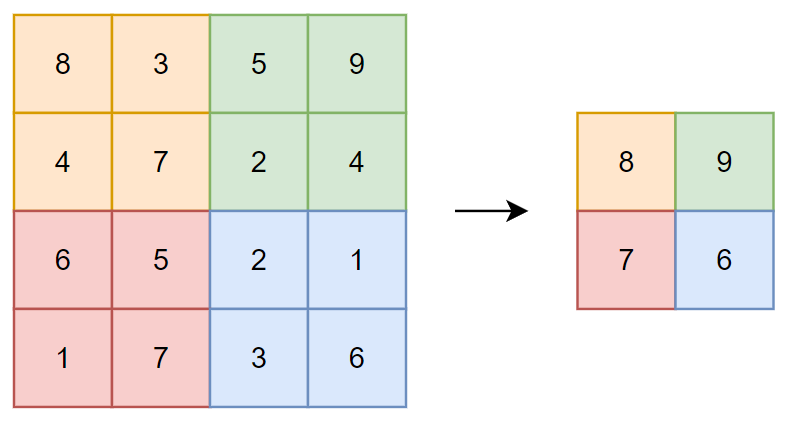
\includegraphics[width=0.5\linewidth]{pooling.png}
    \caption{Max pooling with a filter size of 2 × 2, no padding, and a stride of 2. Adapted from~\cite{Yamashita2018ConvolutionalRadiology}}
    \label{fig:pooling}
\end{figure}

Although max pooling is the most popular type of pooling operations, there is another type called global average pooling. It is an extreme sort of downsampling in which a feature map is downsampled into a 1 x 1 array, by simply taking the average of all the components in each feature map. Before the fully connected layers, this step is usually performed, because it can decrease the number of parameters that may be learned, and it allows the model to take inputs of varying sizes~\cite{Yamashita2018ConvolutionalRadiology}.

After obtaining the feature map of the last convolutional or pooling layer, it is now time to connect it to the fully connected layer. In order to do this, the output needs first to be flattened, or, in other words, needs to be transformed into a one dimensional tensor. After being flattened, the tensor is ready to be fed as input to the fully connected layer and each value of the input is connected to all neurons. 

\paragraph{Recurrent Neural Networks}

In a feedforward neural network, the outputs of one layer are passed to the next layer, which is a unidirectional process. Past data cannot be stored in these feedforward networks~\cite{Shewalkar2019PerformanceGRU}. 

A \gls{RNN} can access previous data because of its loop-like structure, making them ideal algorithms for \gls{ML} supervised challenges involving sequential data, such as speech and handwriting recognition~\cite{Ganatra2018ATools}. Recurrent connections can be generated in \gls{RNN} in three ways: starting in a neuron and ending in the same neuron; starting in a neuron and ending in another neuron from the same layer; or starting in a neuron and ending in another neuron from the previous layer. Only hidden and output neurons establish these recurrent connections; no input or bias neurons are involved. This design allows for the storage of historical data in order to predict current data~\cite{ShewalkarComparisonData}, meaning that it considers both the current input and what it has learnt from previous inputs when making a decision.

\begin{figure}[htbp]
    \centering
    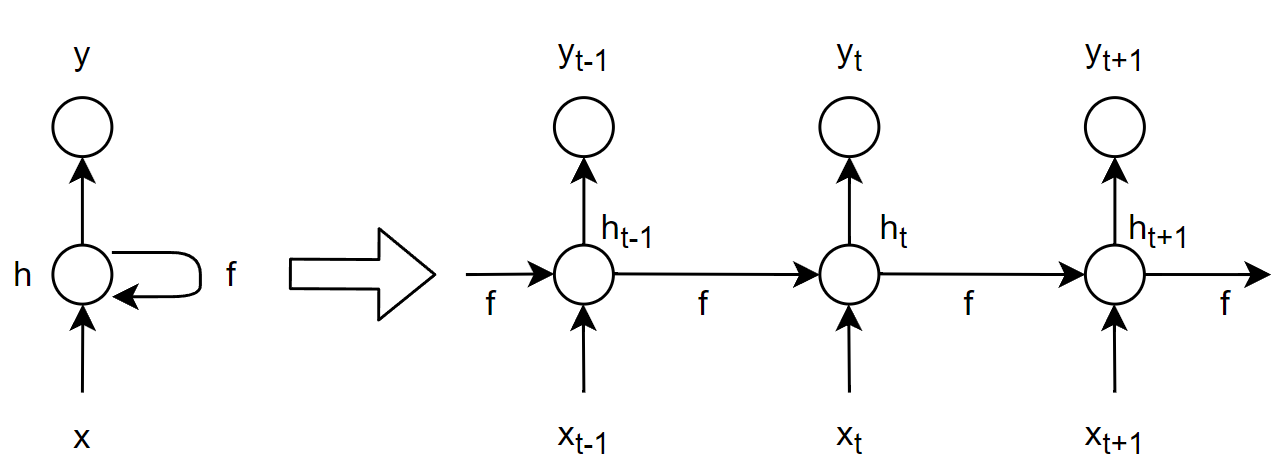
\includegraphics[width=0.75\linewidth]{rnn.png}
    \caption{Recurrent Neural Network architecture. Adapted from~\cite{Gupta2017RecurrentLearning}}
    \label{fig:rnn}
\end{figure}

However, \gls{RNN}s suffer from the vanishing gradients problem, which makes learning large data sequences difficult. Gradients carry the information that is utilized in \gls{RNN} parameter updates, and as they backpropagate through time, they become smaller and smaller. The parameter updates then become so tiny that no significant learning has taken place. Specific \gls{RNN} designs, such as the \gls{LSTM} and \gls{GRU}, were created to overcome the problem of vanishing gradients.

\gls{LSTM} is a \gls{RNN} architecture that was created to more precisely model temporal sequences and their long-range dependencies. \gls{LSTM}s have a similar architecture to RNNs, with the exception that they employ a separate function to calculate hidden state in addition to the gating mechanism. To regulate the information passing through, it has three gates: an input gate, a forget gate, and an output gate. In \gls{LSTM}s, there is a cell that saves past values and keeps them until a forget gate orders the cell to forget them. In another sense, it preserves earlier iterations for as long as they are required. An input gate adds a new input to the cell, while an output gate determines when the vectors from the cell should be sent through to the next hidden state~\cite{Khan2019RNN-LSTM-GRUTransformation}. Each gate is controlled by weights in the cell. The training algorithm, which is usually referred to as \gls{BPTT}, optimizes these weights depending on the network output error~\cite{Madhavan2021DeepDeveloper}.

\gls{GRU}s are a simpler \gls{RNN} architecture with only two gates, the rest gate and the update gate. The rest gate is used in a model to determine how much information from the past should be forgotten or remembered. It decides which information to forget based on the information in the previous state and the next input candidate. The update gate aids the model in determining how much information from previous time steps should be passed on to future time steps.

\gls{GRU} is a simple version \gls{LSTM}, so it can be trained faster, and can execute tasks more efficiently. The \gls{LSTM}, on the other hand, is more expressive, and with more data, it can provide better performance.

\paragraph{Autoencoders}

Autoencoder is an unsupervised neural network that learns how to compress and encode data effectively before reconstructing it back to a representation that is as similar to the original input as possible~\cite{LopezPinaya2020Autoencoders}.

\begin{figure}[htbp]
    \centering
    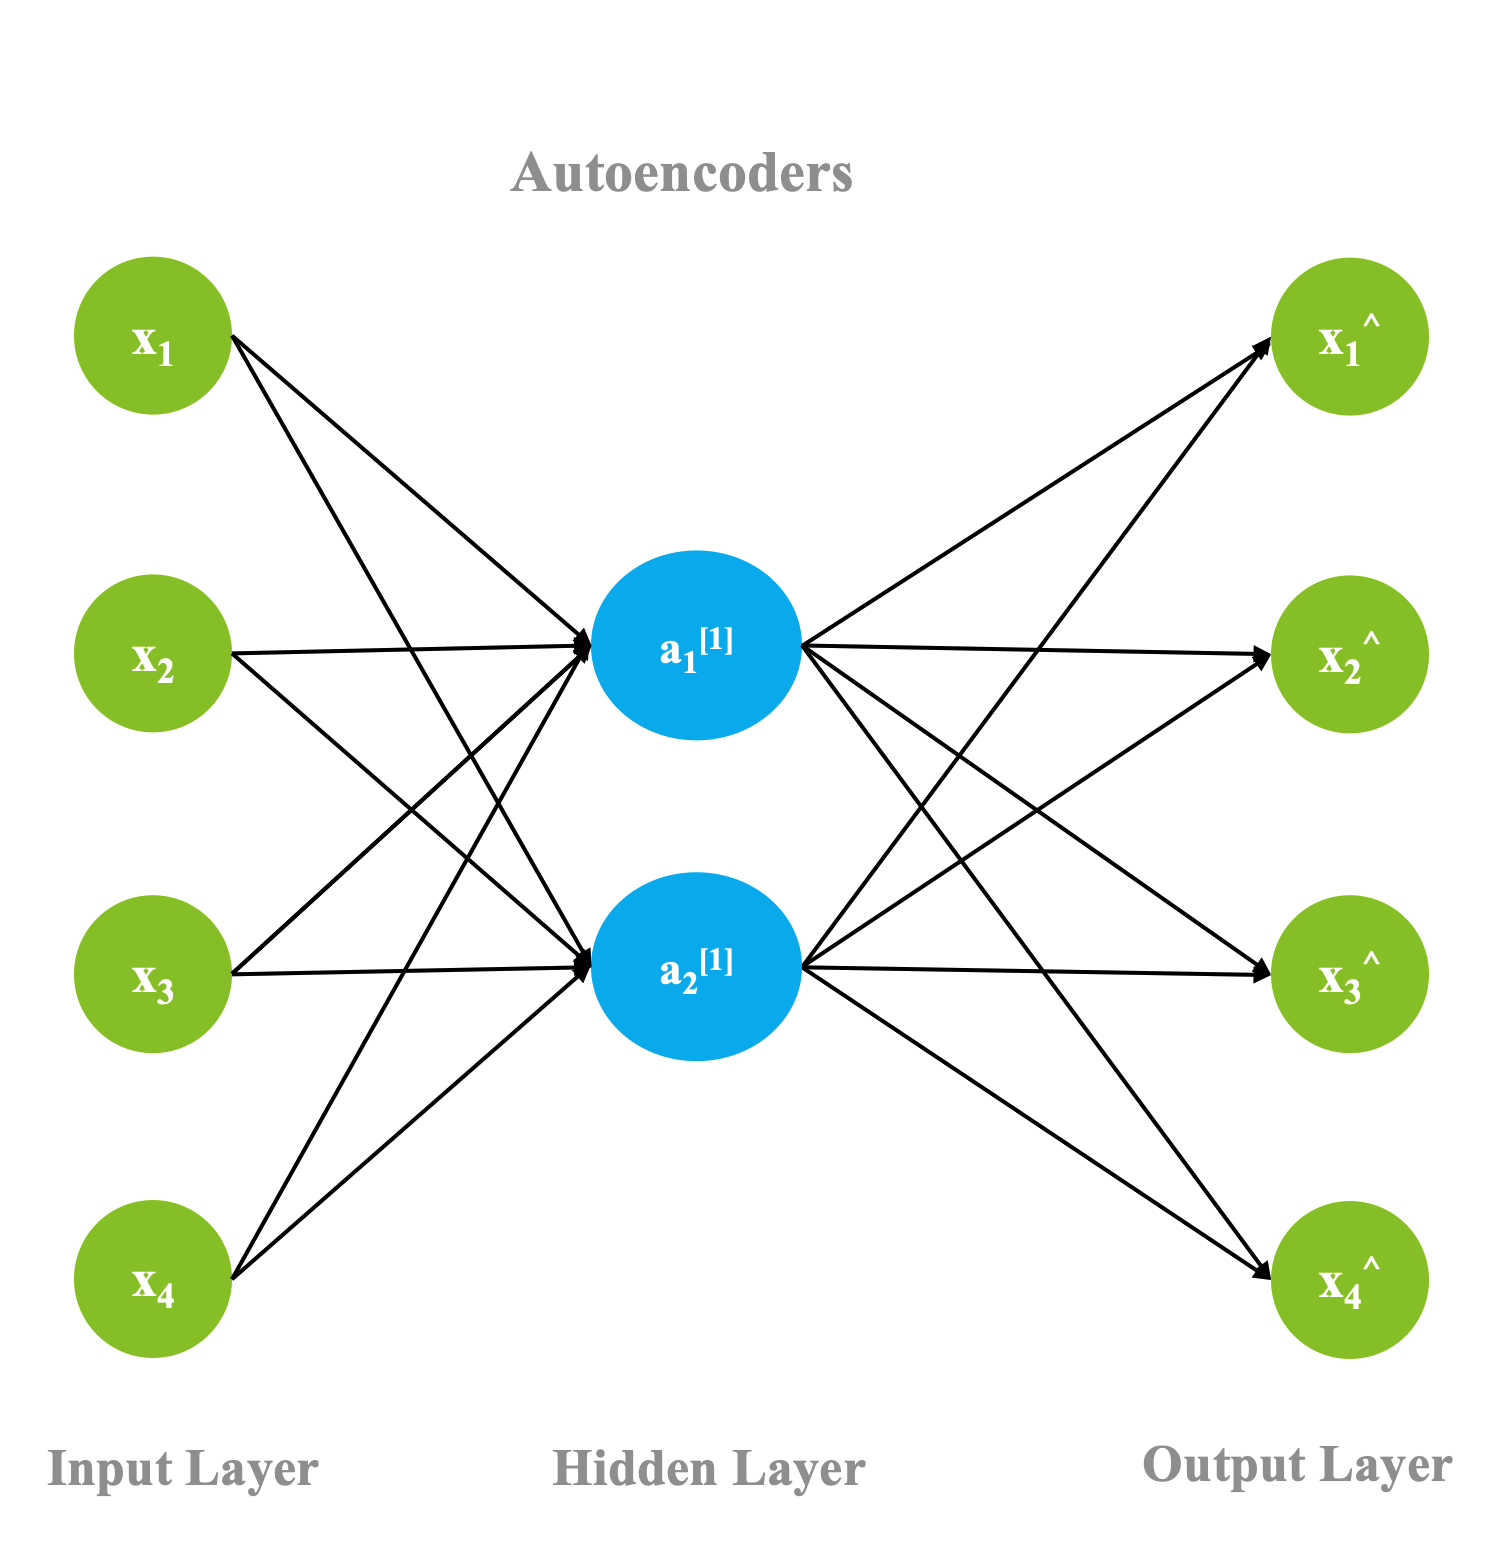
\includegraphics[width=0.5\linewidth]{autoencoders.png}
    \caption{Autoencoders architecture. Adapted from~\cite{Madhavan2021DeepDeveloper}}
    \label{fig:autoencoders}
\end{figure}

As shown in Figure~\ref{fig:autoencoders}, this type of neural network is made up of three layers: input, hidden, and output. First, a suitable encoding function is used to encode the input layer into the hidden layer. The hidden layer contains a significantly smaller number of nodes than the input layer. The compressed form of the original input is stored in this hidden layer. Using a decoder function, the output layer attempts to recreate the input layer. 

As a result, autoencoders consists of 4 main parts~\cite{Abirami2020Energy-efficientSystem,LopezPinaya2020Autoencoders}:

\begin{itemize}
    \item \textbf{Encoder}: The model learns how to compress the input data into an encoded form by reducing the input dimensions.
    \item \textbf{Bottleneck (latent space)}: The compressed form of the input data is stored in this layer. This is the smallest input data dimension imaginable.
    \item \textbf{Decoder}: The model learns how to reconstruct data from the encoded representation as closely as possible to the original input.
    \item \textbf{Reconstruction Loss}: This is a way for determining how well a decoder works and how near the output is to the original input. Back propagation is then used in the training to reduce the network's reconstruction loss.
\end{itemize}

The compressed form of the original input must only have essential information. In other words, an autoencoder can reduce data dimensionality by learning to ignore noise from the input data. 

\section{Automated machine learning}

While \gls{ML} has several proven benefits, its effective use needs a significant amount of work on the part of human specialists, since no algorithm can achieve good performance on all possible challenges. Despite their familiarity with data, researchers frequently lack the \gls{ML} ability required to apply these approaches to large data sets. Researchers can and do collaborate with professional data scientists, but the collaborative approach involves time and effort from both parties. As a result, devising and deploying \gls{ML} solutions is complex, as the process starts with a lengthy data supply procedure, continues with identifying the suitable collaborators, and requires constant back-and-forth between \gls{ML} professionals and domain experts. By automating some of the components that need human skill, sectors will be able to create, verify, and deploy \gls{ML} systems more quickly~\cite{Waring2020AutomatedHealthcare}. As a result, \gls{AutoML} has arisen with the goal of automatically optimizing sections of the \gls{ML} pipeline, such as feature engineering, model selection, and hyperparameter optimization, as shown in Figure~\ref{fig:automl}. 

\begin{figure}[htbp]
    \centering
    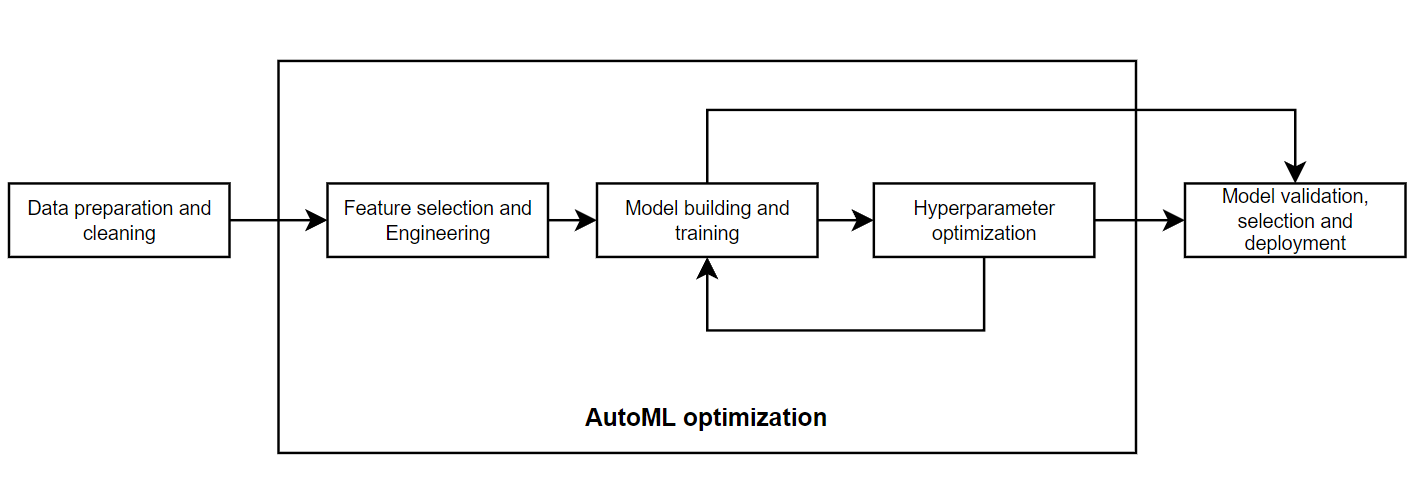
\includegraphics[width=\linewidth]{automl.png}
    \caption{Machine learning pipeline with AutoML. Adapted from~\cite{Waring2020AutomatedHealthcare}}
    \label{fig:automl}
\end{figure}

In recent years, multiple packages have been developed that provide \gls{AutoML}. Some examples are:

\begin{itemize}
    \item \textbf{AutoWEKA} - package for selecting a \gls{ML} algorithm and its hyperparameters at the same time; when paired with the WEKA package, it produces good models for a wide range of data sets automatically.
    
    \item \textbf{Auto-PyTorch} - it is based on the PyTorch \gls{DL} framework and it optimizes the network architecture and training hyperparameters together and reliably to allow fully automated \gls{DL}.
    
    \item \textbf{TPOT} - data science assistant that uses genetic programming to enhance \gls{ML} pipelines and it is built on top of scikit-learn.
    
    \item \textbf{AutoKeras} - open-source software library for \gls{AutoML}. It is built in Keras and provides methods for searching for \gls{DL} architectures and hyperparameters for models. 
    
\end{itemize}


\section{Python libraries for machine and deep learning}\label{sec:ML_DL_libraries}

While there are many languages to choose from, Python is one of the most developer-friendly \gls{ML} and \gls{DL} programming languages available, and it comes with a large library to suit any use-case or project. Most popular libraries include~\cite{JonssonWaysDevelopment,Paszke2019PyTorch:Library}:

\begin{itemize}
    \item \textbf{Tensorflow}: high-performance numerical computing open source software framework. This library, which was created by Google researchers and engineers, has a strong support for \gls{ML} and \gls{DL}. It works with tensors, which are structures that imitate scalars, vectors, and matrices and allow for calculations between them. This tool's key features include straightforward numerical calculation, deployment on numerous CPUs or \gls{GPU}s, and a robust data visualization interface.
    \item \textbf{Keras}: \gls{DL} framework that provides high-level building blocks for designing practically any type of \gls{DL} model in a far more convenient way than constructing it from the ground up. Keras also enables users to train models on both the CPU and \gls{GPU}.
    \item \textbf{PyTorch}: open-source \gls{ML}/\gls{DL} library created by Facebook and based on Torch. It offers a large number of tools and libraries that assist Computer Vision, \gls{NLP}, and a variety of other \gls{ML} tasks. It enables developers to run Tensor computations with \gls{GPU} acceleration and aids in the creation of computational graphs.
\end{itemize}